\chapter{Estudo de Caso}
\label{estudo de caso}

Neste capítulo será apresentado o projeto e a execução do estudo de caso, as análises dos dados quantitativos e qualitativos e a discussão dos resultados. Isso consiste na elaboração de um protocolo para o estudo de caso, na identificação do problema e na definição das questões e objetivos de pesquisa. O método para coleta dos dados e como eles foram analisados também serão apresentados neste capítulo.

\section{Planejamento do Estudo de Caso}

Segundo \citeonline{yin2001estudo}, o estudo de caso é um conjunto de procedimentos 
pré-especificados para se realizar um estudo empírico que investiga um fenômeno contemporâneo dentro de seu contexto da vida real, especialmente quando os limites entre o fenômeno e o contexto não estão claramente definidos. Uma grande vantagem do estudo de caso é a sua capacidade de lidar com uma ampla variedade de evidências, documentos, artefatos, entrevistas e observações. Além disso, em algumas situações, como na observação participante, pode ocorrer manipulação informal.

Buscando maior entendimento a respeito do estudo de caso proposto, foram criadas algumas perguntas que são fundamentais para o seu entendimento:

\begin{easylist}[itemize]	
	
	& Qual o escopo do estudo de caso?
	& Qual o problema a ser tratado?
	& Qual a questão de pesquisa relacionada a esse problema?
	& Quais são os objetivos a serem alcançados nessa pesquisa?	
	& Como foi a seleção do estudo de caso?
	& Qual é a fonte dos dados coletados nessa pesquisa e qual o método de coleta?
	
	\end{easylist}	
	
Com o objetivo da elucidação do escopo do estudo de caso proposto neste trabalho bem como foi ilustrado na Figura \ref{EscopoEstudoCaso}, foram apresentados, nos capítulos anteriores: um estudo teórico relacionado à métricas de software, verificadores de erro, importância do \textit{dashboard} contratação de serviços de TI por parte da Administração Pública Federal brasileira e de Data \textit{Warehouse}. Adicionalmente foi apresentada uma solução para o monitoramento de Métricas de Código-Fonte com suporte de um ambiente de Data \textit{Warehousing}.



Para  as demais perguntas a serem respondidas, foi estruturado neste trabalho um protocolo de estudo de caso baseado em \citeonline{case-study-template-2008} que é dividido da seguinte maneira:

\begin{easylist}[itemize]

& \textbf{Background - Seção \ref{sec:Background}}: Identificar outros estudos acerca do tópico, definir a questão de pesquisa principal e suas proposições derivadas que serão abordadas por este estudo.

& \textbf{Design - Seção \ref{sec:design}}: Identificar se o projeto de pesquisa é um caso único ou múltiplo bem como seu propósito geral. O estudo de caso
único envolve a estratégia de pesquisa aplicada à compreensão de várias dimensões do
fenômeno com foco em um caso singular enquanto o estudo de caso múltiplo envolve o estudo das mesmas dimensões do fenômeno em mais de um caso simultaneamente.

& \textbf{Seleção - Seção \ref{sec:selecao}}: Apresentar critérios para a seleção do caso e descrição do objeto de estudo a ser analisado.

& \textbf{Fonte e Método de Coleta de Dados - Seção \ref{sec:fonte}}: Identificar os dados que serão coletados, definindo um plano para a coleta e como a informação será armazenada.

& \textbf{Processo de Análise dos Dados - Seção \ref{sec:analise}}: Identificar os critérios para interpretação dos resultados do estudo de caso, relacionar os dados com a questão de pesquisa e elaborar a explicação do encontrado.

& \textbf{Ameaças a validade do estudo de caso - Seção \ref{sec:validade}}: Elicitar tipos de validades aplicáveis a um estudo de caso, baseando-se no trabalho desenvolvido por \citeonline{yin2001estudo}, sendo elas: constructo, interna, externa e confiabilidade.


\end{easylist}

\begin{figure}[h!]
\centering
\includegraphics[keepaspectratio=false,scale=0.5]{figuras/figuras_nilton/EscopoEstudoCaso.eps}
\caption{Escopo do Estudo de Caso}
\label{EscopoEstudoCaso}
\end{figure}

\section{Background}\label{sec:Background}

Esta seção contém referências sobre os trabalhos que antecederam esse estudo de caso dentro de um contexto similar ao que foi apresentado, assim como a própria questão geral de pesquisa a ser respondida com todos os elementos necessários para respondê-la.

\subsection{Trabalhos Antecedentes e Relacionados}

O principal trabalho que antecede essa ideia foi desenvolvido por \citeonline{rego_monitoramento_2014}, no qual a solução para monitoramento de métricas de código fonte utilizando \textit{Data Warehouse} foi desenvolvida.

Anteriormente ao trabalho realizado por \citeonline{rego_monitoramento_2014}, \citeonline{marinescu2005measurement} mostrou em seu trabalho que a utilização de métricas isoladas dificulta a interpretação de anomalias do código, reduzindo a aplicabilidade da medição feita. Além disso, o autor ainda afirma que a métrica por si só não contém informação o suficiente para motivar uma transformação no código que que melhore sua qualidade. Buscando trabalhar nesse contexto, \citeonline{marinescu2005measurement} apresentou o conceito de interpretação das métricas em um nível de abstração maior que o adquirido ao observar apenas o valor da métrica.

Outro trabalho antecedente a ser destacado é a tese desenvolvida por \citeonline{Meirelles2013}, em que se buscou responder como métricas de código-fonte podem influir na atratividade de projetos de software livre e quais métricas devem ser controladas ao longo do tempo. Além disso, \citeonline{Meirelles2013} também inseriu como questão de pesquisa se as métricas de código-fonte melhoram com o amadurecimento dos projetos. Durante a execução de seu trabalho, foi observado que, a partir dos resultados obtidos para cada métrica de
código-fonte em uma análise realizada no código-fonte de trinta e oito projetos de software livre, para uma determinada linguagem de programação, é possível definir um intervalo qualitativo a partir de um determinado percentil ao observar o conjunto de valores que são frequentemente obtidos.

O trabalho de \citeonline{Machini2010} fortemente relaciona-se com este trabalho por ter como objetivo fazer com que as métricas de código-fonte sejam mais facilmente incorporadas no cotidiano dos programadores, apresentando uma maneira de interpretar os valores das métricas através de cenários problemáticos que ocorrem frequentemente durante o desenvolvimento.  

Já o trabalho de \citeonline{Ruiz2005} apresenta um ambiente de \textit{data warehousing} para apoiar a implementação de um programa de medição em uma organização certificada como CMM Nível 2. Além disso, foi concebido um experimento que valida sua arquitetura, onde foram usados dados organizacionais reais. \citeonline{Ruiz2005} aborda três aspectos essenciais: 

\begin{easylist}[itemize]

& A captura de dados, considerando os vários tipos de heterogeneidade.
& A integração, transformação e representação de dados quantitativos do projeto de acordo com a visão organizacional unificada e centralizada.
& A funcionalidade de análise que permite o monitoramento do processo.

\end{easylist}

\citeonline{novello_uma_2006} também utilizou \textit{data warehouse} para monitoramento de métricas no processo de desenvolvimento de software, porém essas métricas não eram de código fonte.

Outros trabalhos relacionados ao conceito de métricas de software utilizados nessa revisão são  \citeonline{Fenton98}, \citeonline{metricsandmodels}, \citeonline{McCabe76}. Outros trabalhos que possuem como tema \textit{data warehousing} foram utilizados durante a revisão bibliográfica, entre eles estão  \citeonline{Inmon2002}, \citeonline{Kimball2002}, \citeonline{neeraj_sharma_2011}. 

\subsection{Questão de Pesquisa}

A questão de pesquisa a seguir foi proveniente do problema da falta de capacidade da administração pública em aferir, de forma sistemática e automatizada, a qualidade interna dos produtos de software adquiridos e desenvolvidos por organizações contratadas, que foi identificado na seção \ref{problema} do capítulo \ref{chap:introdução}. 

\textbf{O uso de um ambiente de \textit{Data Warehousing} para aferição da qualidade interna de software, apoiado por ferramentas de análise estática de código-fonte,  pode assistir ao processo de aferição da qualidade interna em uma organização pública federal?}

Para estruturar a questão de pesquisa foi utilizada a técnica \textit{goal-question-metrics} conforme ilustrado na figura \ref{EstruturaEstudoCaso}. Segundo \cite{Basili96b}, o resultado da aplicação do GQM é a especificação de um sistema de medida destinada a um conjunto especifico de questões e um conjunto de regras para a interpretação dos dados da medição. O GQM é uma estrutura hierárquica que começa com um objetivo que especifica o propósito da medição, objeto a ser medido, questão a ser medida e o ponto de vista de quem a observa. O objetivo é refinado em várias questões, onde para cada questão é definida uma métrica(objetiva ou subjetiva)\cite{Basili96b}. A estrutura do GQM está a seguir.

\textbf{Objetivo 01:} Realizar um estudo de caso na CAIXA onde será analisado a capacidade de aferição da qualidade interna de software do ambiente de Data Warehousing apoiado por ferramentas de análise estática de código-fonte.\\


% Questão 01

\textbf{QE01:} Qual a opinião da equipe do CETEC/GITECGO quanto a detecção de cenários de limpeza de código através da solução DW?

\textbf{Fonte:} Entrevista com membros das equipes da CETEC e da GITECGO.

\textbf{Métrica:} Ótimo, Muito Bom, Bom, Ruim, Muito Ruim, Não possui opinião. \\


% Questão 02

\textbf{QE02: } Qual a opinião da equipe do CETEC/GITECGO quanto a detecção de bugs no código(findbugs) através da solução DW?

\textbf{Fonte:} Entrevista com membros das equipes da CETEC e da GITECGO.

\textbf{Métrica:} Ótimo, Muito Bom, Bom, Ruim, Muito Ruim, Não possui opinião.\\


% Questão 03

\textbf{QE03: } Qual a opinião da equipe do CETEC/GITECGO quanto a detecção de violações de código(PMD) através da solução DW?

\textbf{Fonte:} Entrevista com membros das equipes da CETEC e da GITECGO.

\textbf{Métrica:} Ótimo, Muito Bom, Bom, Ruim, Muito Ruim, Não possui opinião.\\


% Questão 04

\textbf{QE04: } Qual a opinião da equipe do CETEC/GITECGO quanto a visualização dos cenários  de limpeza através do \textit{dashboard}?

\textbf{Fonte:} Entrevista com membros das equipes da CETEC e da GITECGO.

\textbf{Métrica:} Ótimo, Muito Bom, Bom, Ruim, Muito Ruim, Não possui opinião.\\


% Questão 05

\textbf{QE05: } Qual a opinião da equipe da CETEC/GITECGO quanto a visualização de violações de código(PMD) através do \textit{dashboard}?

\textbf{Fonte:} Entrevista com membros das equipes da CETEC e da GITECGO.

\textbf{Métrica:} Ótimo, Muito Bom, Bom, Ruim, Muito Ruim, Não possui opinião.\\


% Questão 06

\textbf{QE06: } Qual a opinião da equipe da CETEC/GITECGO quanto a visualização de bugs(findbugs) através do \textit{dashboard}?

\textbf{Fonte:} Entrevista com membros das equipes do CETEC e da GITECGO.

\textbf{Métrica:} Ótimo, Muito Bom, Bom, Ruim, Muito Ruim, Não possui opinião.\\



% Questão 07

\textbf{QE07: } Em relação a visualizações de erros e violações, qual a opinião da equipe da CETEC/GITECGO do uso do DW em comparação à solução do sonarQube?

\textbf{Fonte:} Entrevista com membros das equipes do CETEC e da GITECGO.

\textbf{Métrica:} Muito Melhor, Melhor, Imparcial, Pior, Muito Pior.\\


% Questão 08

\textbf{QE08: } Existe alguma correlação entre \textit{bugs}, violações e cenários analisados? 

\textbf{Fonte:} Total de \textit{bugs}, violações e cenários de limpeza encontrados pela solução de DW.

\textbf{Métrica:} Coeficiente de correlação Linear.\\


% Questão 09

\textbf{QE09: } É possível provar a corretude dos resultados das análises? 

\textbf{Fonte:} Valores das análises apresentados pela solução de DW e valores das análises apresentados pelas ferramentas FindBugs e PMD utilizadas individualmente.
 
\textbf{Métrica:} Erro quadrático médio.\\

	
\begin{figure}[h!]
\centering
\includegraphics[keepaspectratio=false,scale=0.5]{figuras/figuras_nilton/EstruturaEstudoCaso.eps}
\caption{Estrutura do Estudo de Caso}
\label{EstruturaEstudoCaso}
\end{figure}


\section{Design}
\label{sec:design} 

\citeonline{stake_art_1995} identifica três modalidades de estudos de caso: intrínseco, instrumental e coletivo. 

\begin{easylist}[itemize]

& \textbf{Estudo de caso intrínseco:} Constitui o próprio objeto da pesquisa. O que o 
pesquisador almeja é conhecê-lo em profundidade, sem qualquer preocupação com o desenvolvimento de alguma teoria.

& \textbf{Estudo de caso instrumental:} É desenvolvido para auxiliar no conhecimento 
ou na redefinição de determinado problema. O pesquisador não tem interesse específico no caso, mas reconhece que pode ser útil para alcançar determinados objetivos.

& \textbf{Estudo de caso coletivo:} É para estudar características de uma população. Os casos são selecionados porque se acredita que, por meio deles, torna-se possível aprimorar o conhecimento acerca do universo a que pertencem.

\end{easylist}

Como a busca do entendimento geral sobre o problema de pesquisa foi a partir do estudo de um caso particular, o estudo deste  trabalho se caracteriza como instrumental. Podemos observar que a definição de estudo de caso exploratório de \citeonline{yin2001estudo}, onde é elucidada a visão acurada de um caso particular que pode fornecer uma visão geral do problema considerado, que se equivale a definição de estudo de caso instrumental na nomenclatura de \cite{stake_art_1995}. 

\section{Seleção}
\label{sec:selecao} 

A organização pública selecionada para este estudo de caso foi a CAIXA. O estudo aconteceu mais especificamente na Centralizadora Nacional de Tecnologia da Informação (CETEC) e na Gerência de Filial de suporte Tecnológico de Brasília (GITECBR).

Atividades atribuídas à CETEC:

\begin{easylist}[itemize]

& \textbf{Suporte para o ambiente descentralizado} 

& \textbf{Inventário de recurso no ambiente descentralizado} 

& \textbf{Desenvolvimento e produção de soluções no ambiente descentralizado} 

& \textbf{Gestão de incidentes e mudanças no ambiente descentralizado}

\end{easylist}

Atividades atribuídas à GITECBR:

\begin{easylist}[itemize]

& \textbf{Gestão de incidentes tecnológicos de \textit{software} e \textit{hardware}} 

& \textbf{Suporte tecnológico para canais e unidades da CAIXA} 

& \textbf{Desenvolvimento de soluções e serviços tecnológicos de \textit{software} e \textit{hardware}} 

& \textbf{Comunicação no ambiente descentralizado e externo.}

\end{easylist}

A homologação dos serviços e a aceitação dos S\&SC será facultado à CAIXA, submetendo os programas produzidos pela CONTRATADA a testes em produtos de software especializados para avaliação do desempenho dos mesmos. Atualmente, na CETEC, a solução em homologação, que utiliza as unidades da CAIXA no processo de monitoração de métricas de código-fonte adquiridos por empresas terceirizadas, utiliza a ferramenta SonarQube \footnote{http://www.sonarqube.org/}. Apesar do processo existente estar em fase de homologação, a definição de quais as métricas, indicadores e os seus valores de referência para interpretação, ainda não foi finalizado. Diante disso, as medidas que realmente são utilizadas para o ateste da qualidade interna do produto de \textit{software} entregue estão relacionadas ao número de defeitos e ao índice aceitável de defeitos por ponto de função, conforme pode ser observado na Figura \ref{formula}. O número de pontos de defeitos pode gerar multas para a CONTRATADA conforme o índice de defeitos referenciado na tabela \ref{tab:multa}, porém a multa não exime a CONTRATADA das obrigações de corrigir os erros encontrados, onde ainda as alterações propostas pela CONTRATADA deverão ser efetuadas sem qualquer tipo de ônus financeiro ou a outro projeto para a CAIXA.



\begin{figure}[h!]
\centering
\includegraphics[keepaspectratio=false,scale=0.5]{figuras/figuras_nilton/formula.eps}
\caption{Fórmula de Índice de Defeitos}
\label{formula}
\end{figure}

\begin{table}[!ht]
	\begin{center}


\begin{easylist}[itemize]

\begin{flushleft}
Regras relacionadas à Fórmula de Índice de Defeitos:\linebreak[1] 
\end{flushleft}


& Para arredondamento do valor de “Pd” aplicar-se-á a seguinte regra: se o número constante na segunda casa decimal for superior ou igual a 5, o algarismo da primeira casa decimal será acrescido de 1. Caso contrário, o valor da primeira casa decimal permanece inalterado. (ex: se o resultado do cálculo for igual a 0,18, o valor passará a ser 0,2. Se o resultado do cálculo for igual a 0,13, o valor passará a ser 0,1).

& Caso o índice de defeitos fique superior ao aceitável, que é de 0,2 erro por ponto de função, sensibilizará o indicador de desempenho e aplicará o respectivo percentual de redução, conforme a tabela \ref{tab:multa}.\linebreak[1]  
 
\end{easylist}
	
	\input{tabelas/tabelasNilton/multasdefeitos.ltx} 
	\caption{Multa por defeitos}
	\label{tab:multa}
	\end{center}
	\end{table}	
	\FloatBarrier
	
	
Para o estudo de caso deste trabalho foi analisado o Sistema de Gestão Financeira de Bens e Serviços de Tecnologia da Informação (SIGET) um sistema do portfólio da filial GITECBR desenvolvido na linguagem java. Em cada \textit{release} do projeto a GITECBR recebe um pacote da contratada contendo o código-fonte do sistema. Antes da nova versão do sistema entregue ser implantada em ambiente de homologação de sistemas, ela deve passar pela solução disponibilizada pela CETEC que utiliza o sonarQube. O sonarQube apresenta os defeitos contidos no código-fonte. Com base nos defeitos e no índice aceitável de defeitos, que é de 0,2 erro por ponto de função, o gestor define se a \textit{realease} deve ser rejeitada e se existe alguma multa aplicável conforme a tabela \ref{tab:multa}.    

\section{O Software Analisado}

O Projeto Gestão Financeira de Bens e Serviços de Tecnologia da Informação (SIGET) é um sistema web e foi criado a partir de uma necessidade de negócio da Gerência Nacional Gestão de Ativos de TI (GEGAT) para fornecer informações gerenciais e monitorar as atividades de execução físico-financeira dos contratos e contratação de Tecnologia da Informação da CAIXA.

O SIGET possui as funcionalidades de cadastramento de dados sobre as demandas e contratos de bens e serviços de TI e consulta a relatórios para acompanhamento dessas demandas e desses contratos. O acesso deve ser restrito a usuários autorizados e há níveis de permissão diferenciados.

Os subprodutos gerados constituem-se como artefatos do projeto e do sistema. Tal documentação é importante para a conformidade com os normativos e os controles institucionais da CAIXA e formalização dos acordos entre o gestor negocial e a área responsável pela solução tecnológica.

O SIGET é uma ferramenta auxiliar no aprimoramento da gestão de contratos de ativos de TI, reduzindo a utilização de planilhas e controles paralelos, que aumentam o risco operacional. A GEGAT solicitou o desenvolvimento do sistema em módulos para um melhor controle:

\begin{easylist}[itemize]

& Cadastros Auxiliares: Abrange as funcionalidades relacionadas à manutenção das informações gerais das demandas (cadastro principal);

& Demandas: Abrange as funcionalidades correspondentes à manutenção da demanda, sua reserva orçamentária e suas fases;

& Orçamento: Abrange as funcionalidades que tratam da solicitação, aprovação e autorização de orçamento;

& Rotina Automática: Referente à funcionalidade de concessão automática de alguns perfis de acesso a determinados empregados CAIXA.

\end{easylist}

\section{Fonte dos Dados Coletados e Método de Coleta}
\label{sec:fonte} 

Os dados deste estudo de caso foram coletados através de questionários, entrevistas e resultados gerados pela própria solução de \textit{Data Warehousing} utilizando o código-fonte do sistema SIGET desenvolvido por uma empresa contratada pela CAIXA.

Os registros oriundos do questionários foi utilizado principalmente para dados qualitativos. O questionário traz indagações a respeito da solução de \textit{Data Warehousing} pelo ponto de vista dos membros das equipes da CETEC e da GITECGO, no que diz respeito: à detecção de cenários de limpeza de código, detecção de \textit{bugs}, detecção de violações, ao nível de satisfação da solução, ao nível de satisfação da visualização do \textit{dashboard}.

Dados quantitativos da solução foram coletados ao longo das análises das \textit{releases} do SIGET.


\section{Processo de análise dos dados}
\label{sec:analise} 

A análise de dados coletados durante o estudo de caso foi feita através de 4 etapas:

\begin{easylist}[itemize]	
	
	& \textbf{Categorização: } Organização dos dados em duas categorias - qualitativos e quantitativos. Os dados qualitativos referem-se aos questionários e entrevistas realizados. Os dados quantitativos, por sua vez, referem-se aos valores numéricos da solução de DW. 
	& \textbf{Exibição: } Consiste na organização dos dados coletados para serem exibidos através de gráficos, tabelas e texto para poderem ser analisados. 
	& \textbf{Verificação: } Atestar padrões, tendências e aspectos específicos dos significados dos dados. Procurando assim gerar uma discussão e interpretação de cada dado exibido.
	& \textbf{Conclusão: } Agrupamento dos resultados mais relevantes das discussões e interpretações dos dados anteriormente apresentados.
	
	\end{easylist}	


\section{Ameaças a validade do estudo de caso}
\label{sec:validade} 

\citeonline{yin2001estudo} descreve como principais ameaças relacionadas à validade do estudo de caso as ameaças relacionadas à validade de construção, à validade interna, à validade externa e à confiabilidade. As quatro ameaças definidas por ele, bem como a forma usada nesse trabalho para preveni-las, são descritas da seguinte maneira: 

\begin{easylist}[itemize]	

& \textbf{Validade de constructo: } A validade de construção está presente na fase de coleta de dados, quando devem ser evidenciadas as múltiplas fontes de evidência e a coleta de um conjunto de métricas para que se possa saber exatamente o que medir e quais dados são relevantes para o estudo, de forma a responder as questões de pesquisa \cite{yin2001estudo}. O uso do GQM mitiga a validade de construção, uma vez que estabelece uma lógica entre a questão de pesquisa e as métricas que serão analisadas para respondê-la.

& \textbf{Validade interna: } Para \citeonline{yin2001estudo}, o uso de várias fontes de dados e métodos de coleta permite a triangulação, uma técnica para confirmar se os resultados de diversas fontes e de diversos métodos convergem. Dessa forma é possível aumentar a validade interna do estudo e aumentar a força das conclusões.
A triangulação de dados se dará pelas medidas extraídas do código-fonte por meio da solução de \textit{Data Warehousing} (explicada no capítulo \ref{chap:arquitetura}), pela análise de questionários e pelos dados coletados através de entrevistas.

& \textbf{Validade externa: } \citeonline{yin2001estudo} recomenda a replicação do estudo em múltiplos casos. Por esse ser um caso único, a generalização não poderá ser alcançada. Este trabalho é o primeiro a analisar a solução para o estudo de caso na CAIXA, portanto não há como correlacionar os resultados obtidos a nenhum outro estudo.

& \textbf{Confiabilidade: } Com relação a confiabilidade, \citeonline{yin2001estudo} associa à repetibilidade, desde que seja usada a mesma fonte de dados. Nesse trabalho, o protocolo de estudo de caso apresentado nessa seção, além da disponibilização da base de dados coletados e analisados, garantem a repetibilidade desse trabalho e,  consequentemente, a validade relacionada à confiabilidade.

\end{easylist}	

\section{Execução do Estudo de Caso e Análise dos Dados}
\label{chap:execucao}

Para cada uma das \textit{releases} do SIGET, coletou-se o código-fonte, conforme a disponibilidade, no repositório da CAIXA. Após a obtenção do código-fonte,foi realizado a análise estática cada \textit{release} utilizando as ferramentas analizo, findbugs e PMD. Posteriormente, os resultados das análises foram extraídos, transformados e carregados no ambiente de Data Warehousing proposto no Capítulo \ref{chap:arquitetura}. Dessa forma, foi possível obter:

\begin{easylist}[itemize]

& O intervalo qualitativo para cada uma das Métricas de Código-Fonte por \textit{index} e por \textit{release}; 

& Quantidade de Cenários de Limpeza total, por tipo e por \textit{release}; 

& Classe, nome e recomendação para cada cenário de limpeza; 

& Quantidade de \textit{bugs} total,por tipo, por \textit{index} e por \textit{release};

& Classe, tipo, nome e linha para cada \textit{bug}; 

& Quantidade de violações total,por tipo, por \textit{index} e por \textit{release};

& Classe, tipo, nome e linha para cada violação; 

\end{easylist}

Como demonstrado nas Figuras \ref{dashboardtotal}, \ref{dashboardPMD}, \ref{dashboardFindbugs} e \ref{dashboardCenarios}.

\begin{figure}[h!]
\centering
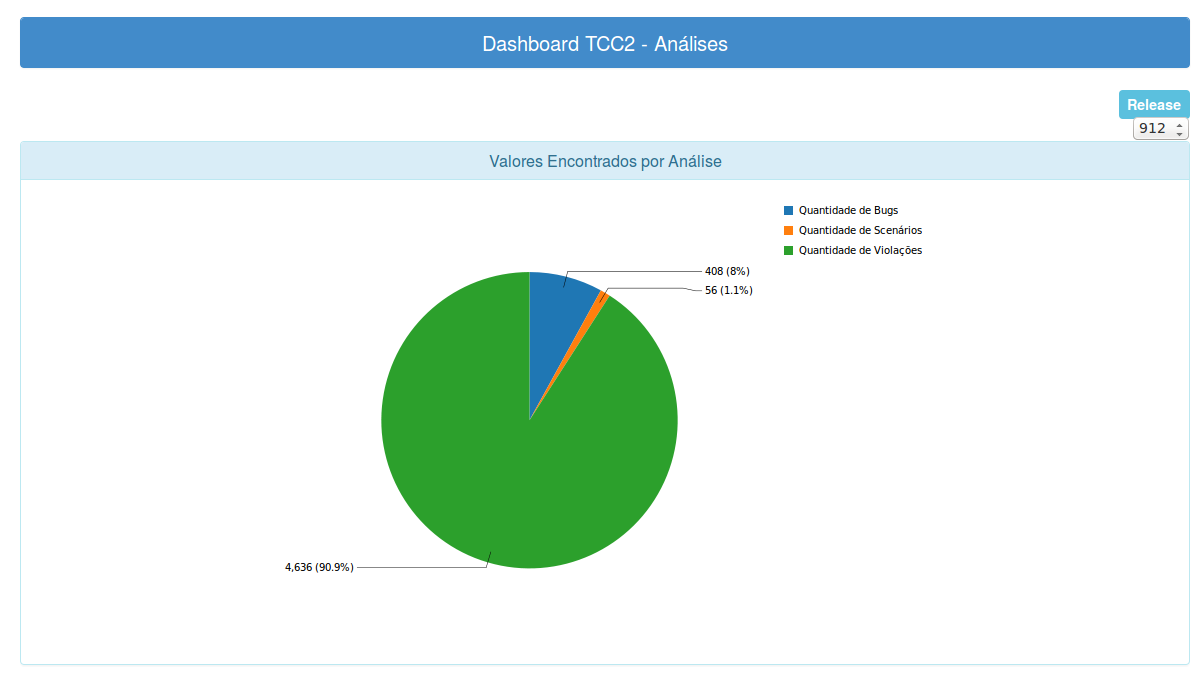
\includegraphics[keepaspectratio=false,scale=0.4]{figuras/figuras_nilton/DashboardTotal.eps}
\caption{\textit{Dashboard} Quantidade Total}
\label{dashboardtotal}
\end{figure}

\begin{figure}[h!]
\centering
\includegraphics[keepaspectratio=false,scale=0.5]{figuras/figuras_nilton/DashboardPMD.eps}
\caption{\textit{Dashboard PMD}}
\label{dashboardPMD}
\end{figure}

\begin{figure}[h!]
\centering
\includegraphics[keepaspectratio=false,scale=0.5]{figuras/figuras_nilton/DashboardCenarios.eps}
\caption{\textit{Dashboard} Cenários}
\label{dashboardFindbugs}
\end{figure}

\begin{figure}[h!]
\centering
\includegraphics[keepaspectratio=false,scale=0.5]{figuras/figuras_nilton/DashboardFindbugs.eps}
\caption{\textit{Dashboard FindBugs}}
\label{dashboardCenarios}
\end{figure}


\subsection{Analise do Erro Quadrático Médio}

Com o objetivo de validar a corretude dos dados apresentados pela solução de DW foi realizado o calculo do EQM (Erro Quadrático Médio). EQM é a soma das diferenças entre
o valor estimado e o valor real dos dados, ponderados pelo número de termos: 

$ EQM = \sum\limits_{i}\frac{(x{i}-y{i})^{2}}{n} $

Quanto mais próximo o valor do EQM de 0, maior a corretude e menor é a diferença entre os valores estimados e os valores reais.

Tomando como referência o valor estimado como os valores apresentados pela a solução de DW e o valor real como os valores apresentados pelas ferramentas \textit{FindBugs} e PMD utilizadas individualmente. Foi calculado o EQM de cada conjunto de regra do FindBugs e do PMD de todas as \textit{releases}, as Figuras \ref{EQMFindBugs}, \ref{EQMPMD1}, \ref{EQMPMD2} e \ref{EQMPMD3} mostram os resultados do EQM. Os valores apresentados pelas ferramentas utilizadas individualmente foram coletados de arquivos do tipo csv por elas geradas, que estão disponíveis para consulta no repositório deste trabalho no \textit{github} \footnote{https://github.com/NiltonAraruna/}. Os valores da solução de DW foram coletados a partir dos \textit{Dashboards} da própria solução. 

As Figuras \ref{comparacaodash} e \ref{comparacaoexcell} exemplificam como os dados foram coletados para o cálculo do EQM. A Figura \ref{comparacaodash} demonstra a quantidade de violações do tipo \textit{Basic} da \textit{release} 914 no \textit{dashboard} do PMD, já a Figura \ref{comparacaoexcell} demonstra a quantidade de violações do tipo \textit{Basic} da mesma \textit{release} no arquivo gerado pela ferramenta PMD.

\begin{figure}[h!]
\centering
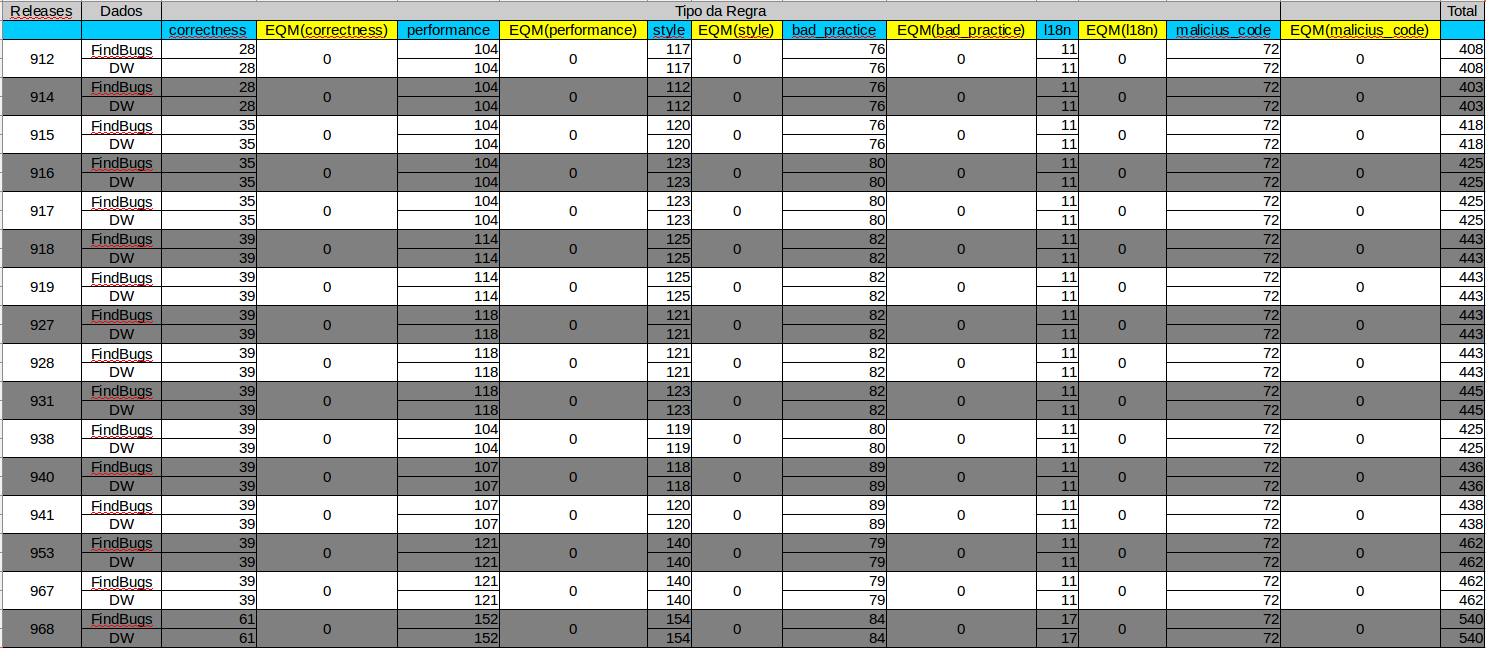
\includegraphics[keepaspectratio=false,scale=0.45,angle=90]{figuras/figuras_nilton/EQMFindBugs.eps}
\caption{\textit{Resultados do EQM do FindBugs}}
\label{EQMFindBugs}
\end{figure}

\begin{figure}[h!]
\centering
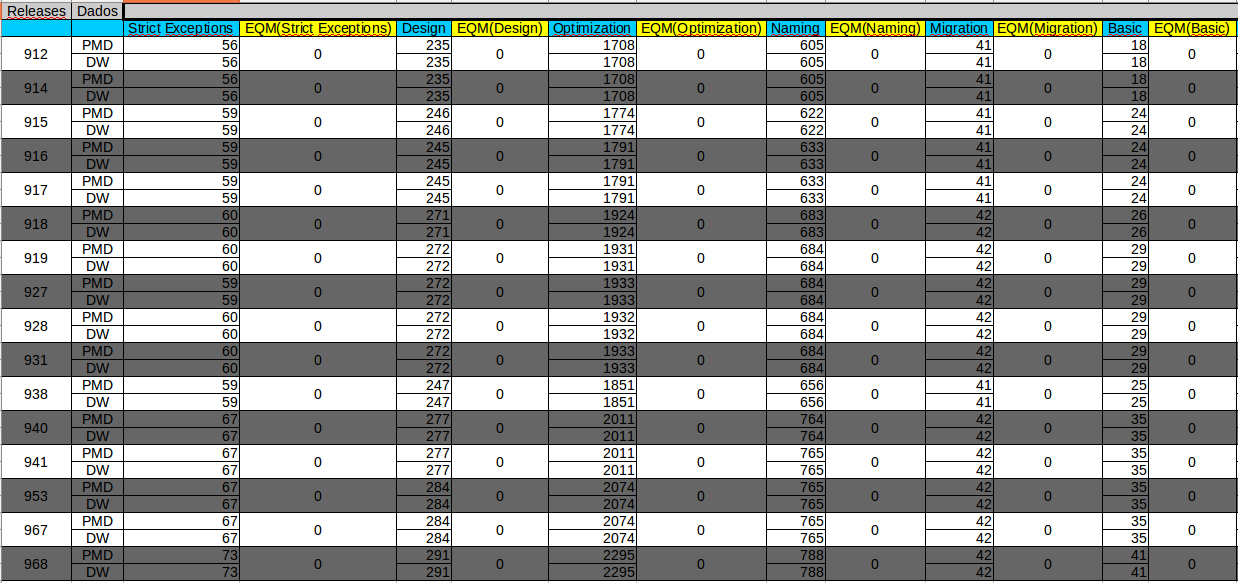
\includegraphics[keepaspectratio=false,scale=0.45,angle=90]{figuras/figuras_nilton/EQMPMD1.eps}
\caption{\textit{Resultados do EQM do PMD}}
\label{EQMPMD1}
\end{figure}

\begin{figure}[h!]
\centering
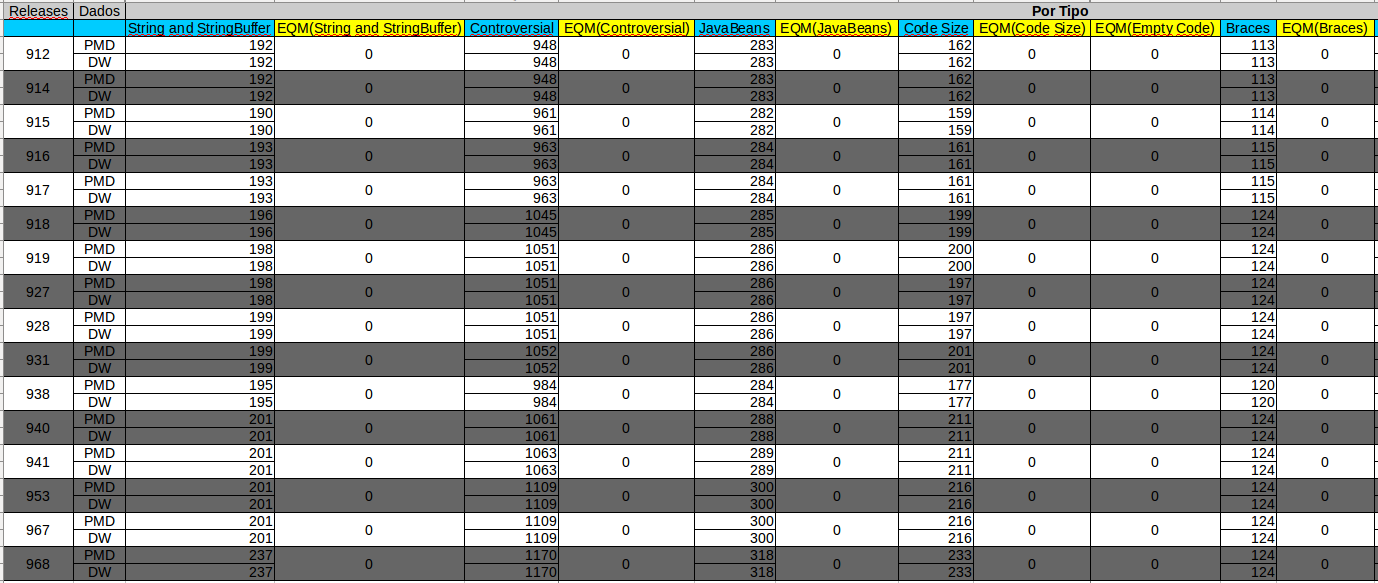
\includegraphics[keepaspectratio=false,scale=0.45,angle=90]{figuras/figuras_nilton/EQMPMD2.eps}
\caption{\textit{Continuação Resultados do EQM do PMD}}
\label{EQMPMD2}
\end{figure}

\begin{figure}[h!]
\centering
\includegraphics[keepaspectratio=false,scale=0.45,angle=90]{figuras/figuras_nilton/EQMPMD3.eps}
\caption{\textit{Continuação Resultados do EQM do PMD}}
\label{EQMPMD3}
\end{figure}

\begin{figure}[h!]
\centering
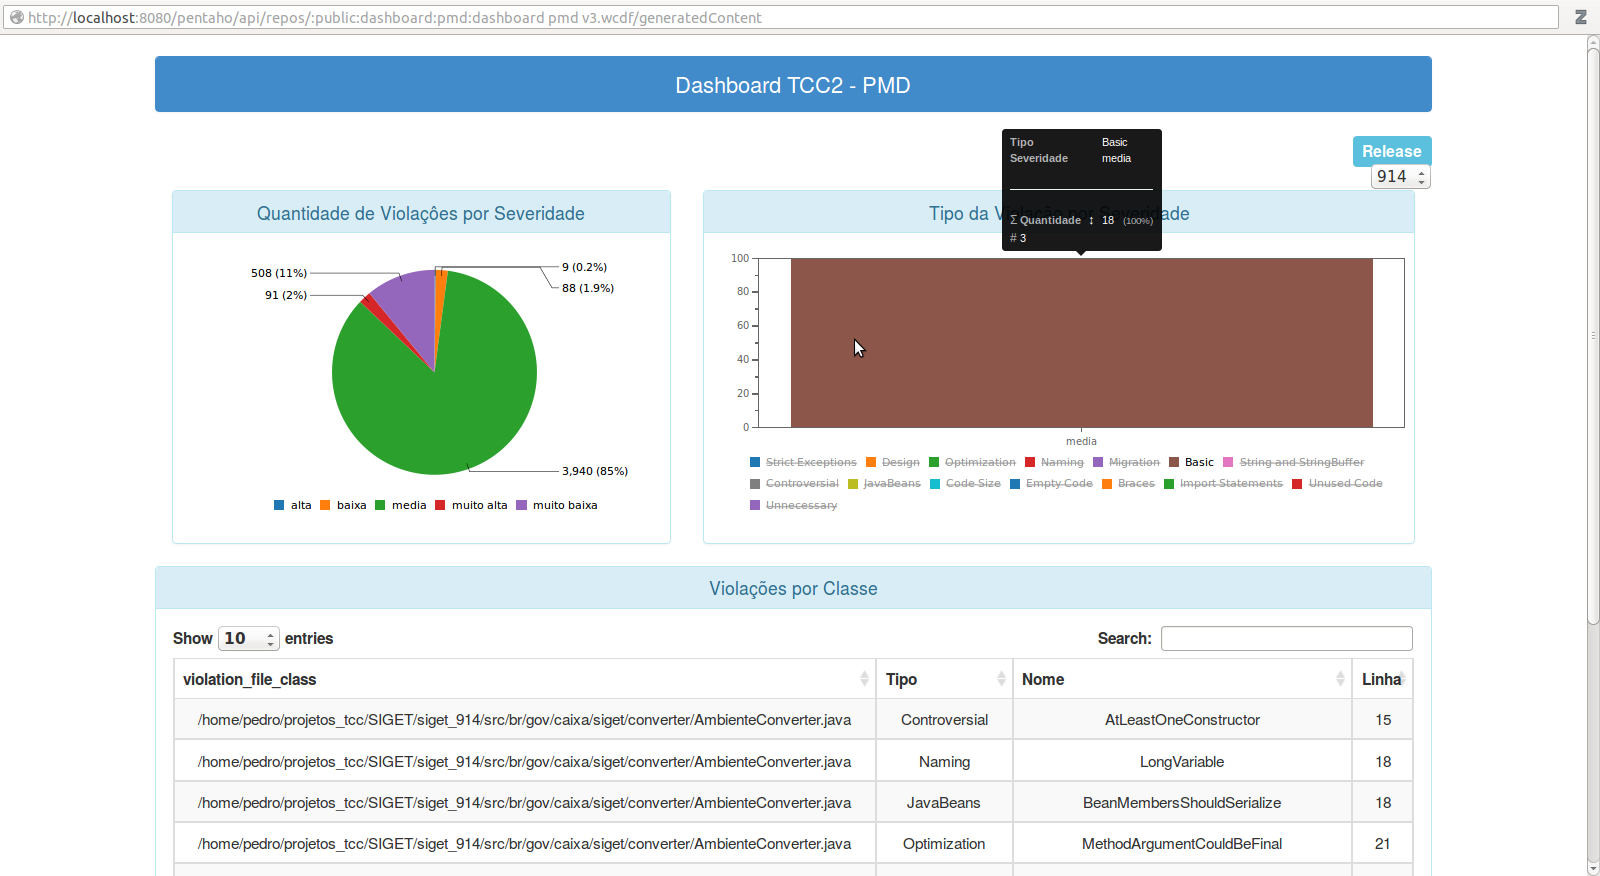
\includegraphics[keepaspectratio=false,scale=0.28]{figuras/figuras_nilton/comparacaodash.eps}
\caption{Exemplo dos dados coletados a partir do \textit{dashboard}}
\label{comparacaodash}
\end{figure}

\begin{figure}[h!]
\centering
\includegraphics[keepaspectratio=false,scale=0.3]{figuras/figuras_nilton/comparacaoexcell.eps}
\caption{Exemplo dos dados coletados a partir do arquivo gerado pela ferramenta PMD}
\label{comparacaoexcell}
\end{figure}

Como pode ser observado os resultados obtidos do EQM foram todos igual a 0, significando a corretude entre os valores obtidos através do \textit{FindBugs} e PMD e os valores apresentados pela solução de DW. A corretude dos valores dos cenários de limpeza não foram validados porque algumas correções e adaptações tiveram que ser feitas na solução de DW de \cite{rego_monitoramento_2014} para que possibilitasse as análises do SIGET, como a adição das função \textit{ROUND} no step "Inserindo os Fatos na $F_Project_Metric $" da transformação "Percentiles Analizo".  


\subsection{Análise do Coeficiente de Correlação}

Segundo \cite{Wasserman2010}, o coeficiente de correlação linear r, proposto por Karl Pearson, é calculado a partir de uma amostra de n pares de observações de X e Y, e mede a intensidade e a direção da relação linear entre duas variáveis quantitativas e o grau de correlação entre as variáveis:

$ r = \frac{\sum(X-X')(Y-Y')}{\sqrt{[\sum(X-X')^{2}][\sum(Y-Y')^{2}]}} $


Correlação entre duas variáveis é quando uma delas está, de alguma forma, relacionada com a outra. A Tabela \ref{tab:correlacao} mostra a significância de índice de Correlação segundo \cite{Wasserman2010}.

\begin{table}[!ht]
	\begin{center}
\input{tabelas/tabelasNilton/correlacao.ltx} 
	\caption{Significância de índice de Correlação}
	\label{tab:correlacao}
	\end{center}
	\end{table}	
	\FloatBarrier

Um diagrama de dispersão também demostra a relação entre duas variáveis quantitativas, medidas sobre os mesmos indivíduos. Se a reta do gráfico for mais próxima de
uma reta de 45 graus, maior será a correlação positiva, se a reta apresentada for mais próxima de 135 graus, maior será a correlação negativa. 

Não querendo generalizar o resultado de uma possível correlação entre \textit{bugs}, violações e cenários de limpeza por se tratar de um estudo de apenas um estudo de caso, uma instituição e um sistema, foi calculado o coeficiente de correlação linear entre \textit{bugs} e violações, entre \textit{bugs} e cenários de limpeza e entre cenários de limpeza e violações. O resultado do cálculo do coeficiente de correlação linear pode ser vista na Figura \ref{correlacao}.

\begin{figure}[h!]
\centering
\includegraphics[keepaspectratio=false,scale=0.40,angle=90]{figuras/figuras_nilton/correlacao.eps}
\caption{Resultado do cálculo do coeficiente de correlação linear}
\label{correlacao}
\end{figure}

Analisando os resultados do coeficiente de correlação linear em conformidade com a Tabela \ref{tab:correlacao} podemos notar que a correlação entre cenários de limpeza e violações, entre violações e \textit{bugs} e correlação entre cenários e \textit{bugs} é uma correlação direta e muito forte. Os gráficos de dispersão das Figuras \ref{dispercaocenariosbugs}, \ref{dispersaocenariosviolacoes} e \ref{dispersaoviolacoesbugs} também demonstra uma correlação direta e muito forte pois as retas dos gráficos se aproximam de 45 graus.

\begin{figure}[h!]
\centering
\includegraphics[keepaspectratio=false,scale=0.40]{figuras/figuras_nilton/dispercaocenariosbugs.eps}
\caption{Gráfico de Dispersão entre Cenários de Limpeza e \textit{Bugs}}
\label{dispercaocenariosbugs}
\end{figure}


\begin{figure}[h!]
\centering
\includegraphics[keepaspectratio=false,scale=0.40]{figuras/figuras_nilton/dispersaocenariosviolacoes.eps}
\caption{Gráfico de Dispersão entre Cenários de Limpeza e Violações}
\label{dispersaocenariosviolacoes}
\end{figure}

\begin{figure}[h!]
\centering
\includegraphics[keepaspectratio=false,scale=0.40]{figuras/figuras_nilton/dispersaoviolacoesbugs.eps}
\caption{Gráfico de Dispersão entre Violações e \textit{Bugs}}
\label{dispersaoviolacoesbugs}
\end{figure}

\subsection{Analise do Questionário}

O questionário aplicado pode ser encontrado no Apêndice \ref{sec:questionário}. Vale ressaltar que esse questionário foi aplicado não só para caracterização do conhecimento sobre qualidade dos envolvidos do estudo de caso na CAIXA como também para coleta de dados qualitativos necessários para responder questões específicas do GQM. 

Das 15 pessoas que realizaram o questionário todas trabalham na CETEC, sendo 4 do núcleo de inovação, 2 do núcleo qualidade, 3 do núcleo de governança, 3 do núcleo de banco de dados, 1 analista, 1 coordenador e 1 gerente de projetos. Do total 46,7\% trabalham na mesma área de atuação entre 3 a 5 anos, 33,3\% a mais de 5 anos e 20\% a menos de 2 anos. 

Em relação a QE01 e QE04: 20\% definiram como Ótimo, 73,3\% como Muito Bom e 6.7\% como sem opinião. Sendo que 80\% dos entrevistados entenderam o conceito sobre cenários de limpeza.

Em relação a QE02: 53.3\% definiram como imparcial, 26.7\% Melhor e 20\% Muito Melhor a solução de DW em relação ao FindBugs. Sendo que 66.7\% nunca utilizaram a ferramenta FindBugs.

Em relação a QE03: 80\% definiram como imparcial, 13.3\% Melhor e 6.7\% Muito Melhor a solução de DW em relação ao PMD. Sendo que 99.3\% nunca utilizaram a ferramenta PMD.

Em relação a QE05 e QE06: 40\% definiram como Ótimo, 46.7\% Muito Bom e 13.3\% Bom a opinião quanto a visualização das análises através do \textit{dashboard} da solução de DW. 

Em relação a QE07: 26.7\% definiram como Melhor e 76.3\% como Imparcial. Sendo que 73.3\% nunca utilizaram a ferramenta sonarQube. 

Pontos fortes da solução de DW levantados pelo questionário:

\begin{easylist}[itemize]

& A forma pratica na apresentação dos \textit{bugs};

& Apresentação de Cenários de limpeza;

& Apresentação de informações de forma direcionada;

& Simplicidade na visualização;

& Apresentar de forma gráfica os \textit{bugs}, violações e cenários de limpeza detectados e auxiliar na tomada de decisões;

& Possibilidade de trabalhar com grande diversidade de dados;

& Concentrar os dados em um local proporcionando novas analises;

& Permitir a prevenção dos sistemas já em produção e agregar qualidade nas aferições por parte da empresa pública;

& Uma visão gerencial, Ferramental que auxilia na tomada de decisões;

& Traduz de forma simples os resultados das análises, facilitando o dia a dia do usuário;

& Dar visibilidade quanto a qualidade dos produtos entregues e auxiliar na tomada de decisões.

\end{easylist}


Pontos fracos da solução de DW levantados pelo questionário:

\begin{easylist}[itemize]

& Caso precise, a manutenção seria custosa  e teria que ter uma equipe com conhecimentos técnicos sobre a solução;

& Recomendações para violações e \textit{bugs};

& Layout mais atrativo e recomendações conceituais;

& Tempo necessário para visualização das análises; 

& Detalhar melhor as recomendações para os cenários de limpeza;

& Necessidade de outras ferramentas para fazer as análises.

\end{easylist}

De todos que responderam o questionário, 100\% definiram que a solução de DW traria benefícios para a CAIXA, benefícios apontados:

\begin{easylist}[itemize]

& Com a visualização de \textit{bugs}, violações e cenários de limpeza a Caixa teria maior visibilidade da qualidade dos softwares que são entregues pelas tercerizadas;

& Agilidade na validação e refatoração do código;

& Melhora na identificação do nível de qualidade dos produtos entregues pelas fábricas de software;

& Apoio na devolução de entregas com inconsistências para a fábrica e na aplicação de multas.

& Visualização do Percentual de \textit{bugs}, violações e cenários de limpeza encontrados nas aplicações;

& Apresenta maior quantidade de informações que outras ferramentas;

& A solução apoia a melhoria contínua da qualidade;

& Automação da validação de código-fonte;

& O ganho da qualidade do software entregue

& Agregar qualidade nos recebimentos.

& Facilidade na visualização e acesso a dados importantes para a refatoração;

& Apoio na aferição de qualidade dos projetos desenvolvidos pelas fábricas que hoje está abaixo da média esperada.

\end{easylist}

\section{Considerações finais do capítulo}

Esse capítulo teve como objetivo apresentar o protocolo de estudo de caso que foi adotado neste trabalho, sua execução, as análises dos dados quantitativos e qualitativos e a discussão dos resultados. No próximo capítulo será apresentado a conclusão, limitações e trabalhos futuros.